\section{Discussion}

The results of our experimentation demonstrate the efficacy of transfer learning and hyperparameter optimization in developing a robust mushroom classification model. By systematically exploring different configurations, we were able to improve the model's performance and mitigate misclassifications, particularly focusing on correctly identifying poisonous mushrooms.
Even though we were able to get a good result with such challanging dataset,deep learning faces numerous challenges, that includes overfitting, vanishing/exploding gradients, lack of interpretability, and data efficiency\cite{alzubaidi2021review}. We tried to see what the filters are seeing in convolution layer. We took 3 filters from beginning layer, middle layer and last layer.
The filters from first convolution layers were looking to find global pattern in the images. It tries to learn from the whole picture.
\begin{figure}[h]
    \centering
    \begin{subfigure}[b]{0.3\textwidth}
        \centering
        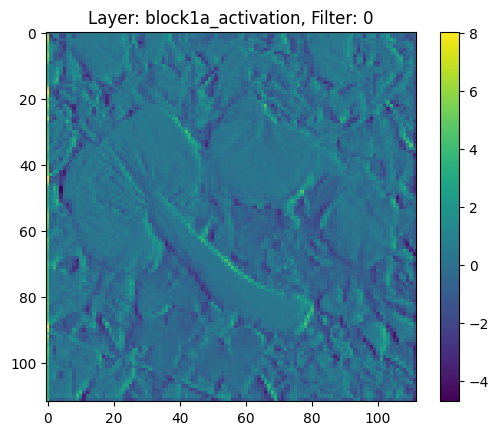
\includegraphics[width=\textwidth]{images/filter 0block1a_activation.png}
        \caption{Filter 1}
        \label{fig:filter1}
    \end{subfigure}
    \begin{subfigure}[b]{0.3\textwidth}
        \centering
        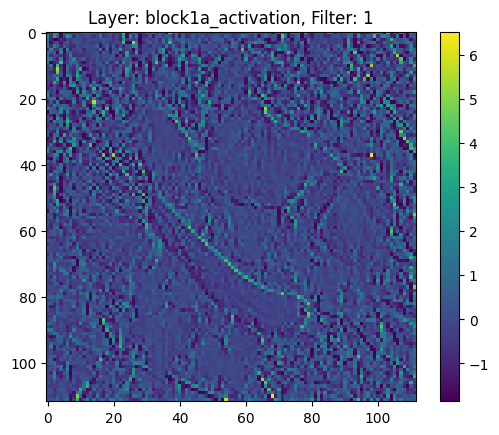
\includegraphics[width=\textwidth]{images/filter 1block1a_activation.png}
        \caption{Filter 2}
        \label{fig:filter2}
    \end{subfigure}
    \begin{subfigure}[b]{0.3\textwidth}
        \centering
        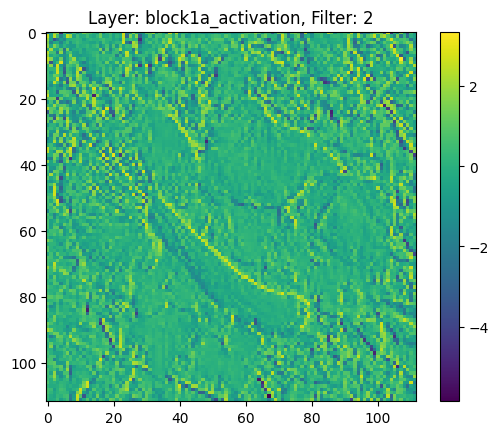
\includegraphics[width=\textwidth]{images/filter 3block1a_activation.png}
        \caption{Filter 3}
        \label{fig:filter3}
    \end{subfigure}
    \caption{Filters from the first convolutional layer}
    \label{fig:conv_filters}
\end{figure}

Similarly, 3 filters from block 6 convolution layer were viewed those patterns are hard to be understood by humans. This shows that the deep learning has the challange of interpretability.
\begin{figure}[h]
    \centering
    \begin{subfigure}[b]{0.3\textwidth}
        \centering
        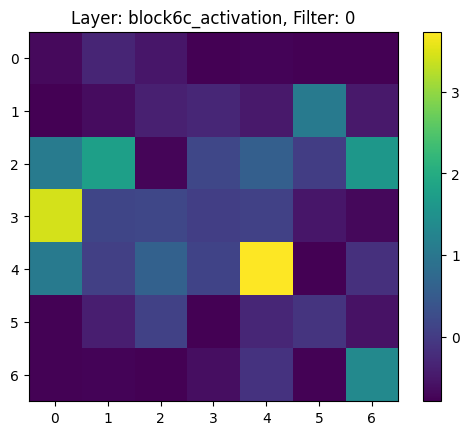
\includegraphics[width=\textwidth]{images/filter 0block6a_activation.png}
        \caption{Filter 1}
        \label{fig:filter1}
    \end{subfigure}
    \begin{subfigure}[b]{0.3\textwidth}
        \centering
        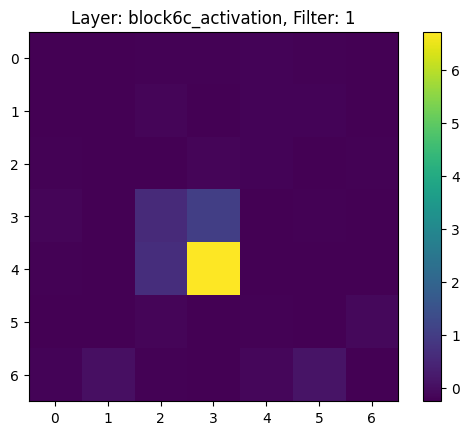
\includegraphics[width=\textwidth]{images/filter 1block6a_activation.png}
        \caption{Filter 2}
        \label{fig:filter2}
    \end{subfigure}
    \begin{subfigure}[b]{0.3\textwidth}
        \centering
        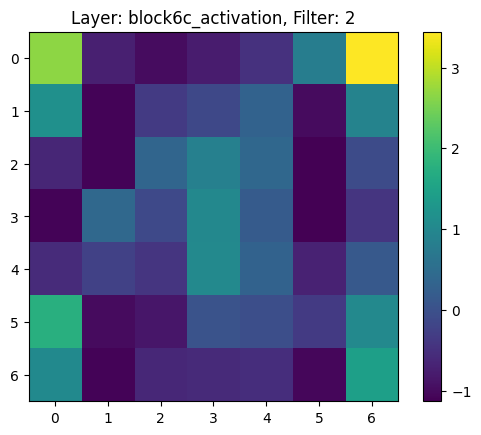
\includegraphics[width=\textwidth]{images/filter 2block6a_activation.png}
        \caption{Filter 3}
        \label{fig:filter3}
    \end{subfigure}
    \caption{Filters from the sixth convolutional layer}
    \label{fig:conv_filters}
\end{figure}

We also tried to visualise what the top activation layer is seeing before deciding to classify the mushroom. Here as well interpretation is difficult.
\begin{figure}[h]
    \centering
    \begin{subfigure}[b]{0.3\textwidth}
        \centering
        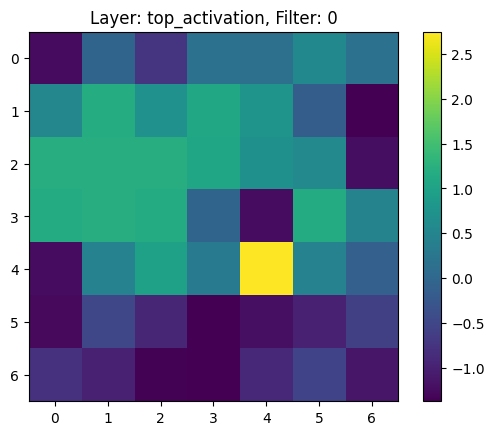
\includegraphics[width=\textwidth]{images/filter0 top_activation.png}
        \caption{Filter 1}
        \label{fig:filter1}
    \end{subfigure}
    \begin{subfigure}[b]{0.3\textwidth}
        \centering
        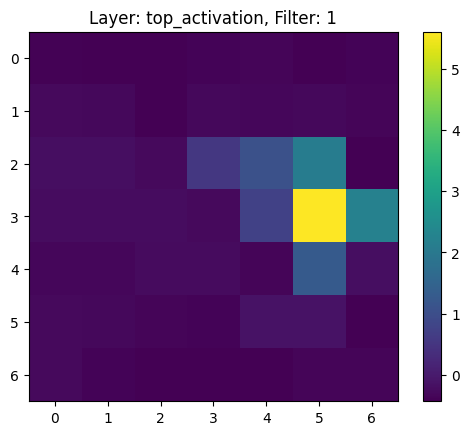
\includegraphics[width=\textwidth]{images/filter1 top_activation.png}
        \caption{Filter 2}
        \label{fig:filter2}
    \end{subfigure}
    \begin{subfigure}[b]{0.3\textwidth}
        \centering
        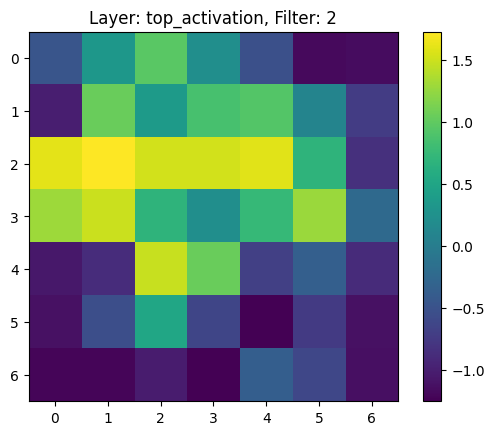
\includegraphics[width=\textwidth]{images/filter2 top_activation.png}
        \caption{Filter 3}
        \label{fig:filter3}
    \end{subfigure}
    \caption{Filters from the top activation layer}
    \label{fig:conv_filters}
\end{figure}

The comparison of our model's performance on the additional dataset underscores the importance of appropriate data division and validation techniques in assessing model generalization and robustness. While the previous study reported impressive accuracy and recall rates, our adjustment to the data division revealed potential vulnerabilities in the model's classification capabilities. By allocating a portion of the dataset for validation accuracy checking and adopting a more balanced data division approach, we were able to achieve superior performance, accurately classifying all poisonous mushrooms and mitigating the risk of misclassification. This emphasizes the critical role of rigorous validation and evaluation methodologies in ensuring the reliability and efficacy of machine learning models in real-world applications.


The utilization of EfficientNetB0, a state-of-the-art convolutional neural network architecture, played a pivotal role in achieving high classification accuracy. Its ability to capture intricate features and patterns in mushroom images, despite their diverse colors and shapes, underscores its suitability for complex classification tasks.



Our study also sheds light on the challenges posed by diverse and unaltered datasets, contrasting with previous studies that often relied on augmented datasets for training. Despite these challenges, our model demonstrated competitive performance, showcasing the robustness of transfer learning in handling real-world datasets with inherent variability.


Furthermore, our research highlights the potential practical applications of such models beyond mushroom classification. The development of a mobile application incorporating this technology could serve as a valuable tool for outdoor enthusiasts, providing guidance on identifying edible and poisonous vegetation and fruits during outdoor expeditions or in survival situations.

Overall, our study contributes to the growing body of research on machine learning applications in mycology and underscores the potential for broader applications in related fields such as food safety, environmental conservation, and public health. Future research could explore additional techniques for dataset augmentation, further refine model architectures, and extend the classification framework to encompass a broader range of toxic vegetation and fruits for enhanced utility in real-world scenarios.